\documentclass[twoside,leqno,twocolumn]{article}
\usepackage[letterpaper]{geometry}
\usepackage{ltexpprt}
\usepackage{amsmath,amssymb,graphicx,booktabs,url}
\title{\Large Cross-Checking Serialized Tetrahedral Meshes with Analytic Volumes and Boundary Incidence\\[0.4em]\normalsize Author-review draft; not submitted}
\author{}
\date{}
\begin{document}
\maketitle
\begin{abstract}
A native mesher's successful return does not by itself establish that every element was checked or that the published file preserves the intended mesh. This research note presents a bounded STEP-to-tetrahedron verification example using two analytic reference solids at three fixed size settings. The maintained adapter checks every element's sampled signed inverted condition number in bounded batches before publishing a result. An independent ASCII MSH 4.1 reader then reconstructs tetrahedral volumes, face and edge incidence, connected components and Euler counts from the retained files without importing the mesher. All six existing meshes reproduce their retained volumes and element counts. Their serialized surface triangles equal their tetrahedral boundaries; the box has solid/boundary Euler values 1/2 and the drilled plate 0/0. Plate volume error ranges from 0.154483\% to 0.526629\%, while the box volume is exactly 1000 mm$^3$ at reported precision. The artifact is a small reproducible verification example. It does not establish industrial coverage, geometric embeddedness, solver convergence, structural safety or learned-generation quality.
\end{abstract}

\section{Problem and Contribution}
Mesh generation and mesh publication are different operations. An adapter can successfully invoke a native mesher yet omit an element-quality query, aggregate batches incorrectly, or publish serialized data that does not match its receipt. Reference geometries with known volume make these failure modes easier to examine because the expected measurement does not depend on a downstream simulation.

This note studies a narrow engineering question: do native tetrahedral meshes of a box and a through-hole plate satisfy the declared quality, serialization and reference-volume checks, and do independent combinatorial diagnostics agree with the expected solid types? The contribution is a reproducible combination of existing checks and controlled examples, not a new meshing algorithm. The native generator is Gmsh~\cite{gmsh2009}; its quality query and MSH semantics follow the reference manual~\cite{gmshmanual}.

The retained implementation previously skipped quality queries above 200,000 volume elements, although its mesh-size ceiling was 2,000,000. The corrected adapter queries all elements in batches of at most 200,000. A result is rejected if a batch has missing, nonfinite or nonpositive quality values. The global mean is accumulated by element count, including an uneven final batch. Fault-injection tests exercise this boundary using reduced batch limits; the six native examples themselves contain 643--5,033 tetrahedra. No large-mesh performance result is inferred from them.

\section{Reference Geometry and Native Evidence}
The box measures $20\times10\times5$ mm, giving an analytic volume of $1000$ mm$^3$. The plate measures $20\times12\times4$ mm and contains a central radius-2 mm cylindrical through-hole, giving
\begin{equation}
 V_{\rm plate}=20\cdot12\cdot4-\pi(2^2)\cdot4=960-16\pi.
\end{equation}
The retained protocol uses maximum mesh sizes $h\in\{4,2,1\}$ mm, with minimum size $h/5$. The fixed relative-volume tolerances are $10^{-9}$ for the box and 2.5\% for the plate. They were specified in the reference runner before the retained execution. No tolerance is tightened or selected using the new analysis.

Gmsh's OpenCASCADE kernel constructs a single solid and exports STEP. The maintained adapter then imports the STEP snapshot, creates the tetrahedral mesh and serializes MSH plus a receipt. The original environment records Gmsh 4.15.2, NumPy 2.3.5 and Python 3.12.14. Each receipt binds the consumed STEP bytes and produced mesh bytes. The aggregate report also records the source file digests used in that execution.

The quality measure is Gmsh's sampled minimal signed inverted condition number, \texttt{minSICN}. This note reports the retained minima and means; the new reader does not independently reproduce Gmsh's quality formula. In contrast, oriented tetrahedral volumes are independently recomputed from serialized coordinates. For vertices $a,b,c,d$,
\begin{equation}
 V_t=\frac{1}{6}\det[b-a,\ c-a,\ d-a].
\end{equation}
Every retained tetrahedron must have finite positive oriented volume. The sum uses stable floating-point accumulation and is compared with the analytic part volume. Positive local determinants are necessary diagnostics; they do not exclude intersections between unrelated tetrahedra.

\section{Independent Serialized-Mesh Analysis}
The added analysis consumes the six existing MSH files without rerunning Gmsh. Before reading them, it verifies all 16 files named by the original artifact manifest. It therefore analyzes the retained campaign rather than creating a replacement campaign.

The reader accepts an intentionally narrow subset: ASCII MSH 4.1, nonparametric node blocks and linear simplices. It checks section uniqueness, declared counts, positive unique tags, finite coordinates and valid connectivity. Unsupported formats and element types fail explicitly. A separate test suite includes inverted and duplicate tetrahedra, missing nodes, nonfinite coordinates, mismatched surface triangles and inconsistent shared-face orientation.

\subsection{Incidence and orientation}
For each positive tetrahedron, the reader enumerates its four outward-oriented triangular faces. A sorted node triple is the face key; a permutation parity records its orientation. Interior faces must have two owners with opposite orientation. Faces with one owner form the derived boundary. Faces with more owners or equal interior orientation are rejected.

The derived boundary must match the unordered set of serialized surface triangles exactly, without duplicates. Each boundary edge must appear twice with opposite orientation. Two adjacency graphs then count connected components: tetrahedra are adjacent across interior faces, and boundary triangles are adjacent across shared edges. These diagnostics expose several serialization and incidence inconsistencies without depending on a second call to the mesher.

\subsection{Euler diagnostics}
The volume complex has counts $V,E,F,T$, giving
\begin{equation}
 \chi_{\rm solid}=V-E+F-T.
\end{equation}
Its boundary has counts $V_b,E_b,F_b$, giving $\chi_{\partial}=V_b-E_b+F_b$. The analytic box is ball-like and has expected values 1 and 2. The through-hole plate is solid-torus-like and has expected values 0 and 0. These values are compared alongside one connected volume component and one connected boundary component.

Matching Euler values is not a classification theorem for the mesh. The checker does not test every vertex link, detect arbitrary element intersections, establish a homeomorphism with the CAD solid or prove exact embedding. For this reason the output calls them topology diagnostics, not a general topology-completeness certificate.

\begin{table*}[t]
\centering
\caption{All six retained meshes pass the independent analysis. $h$ is the maximum size in mm. Volumes are mm$^3$. SICN is the retained native value; all other listed mesh counts and volumes are recomputed from ASCII connectivity and coordinates.}
\label{tab:results}
\begin{tabular}{lrrrrrrrr}
\toprule
Part & $h$ & Vertices & Tetrahedra & Mesh volume & Rel. error (\%) & Min. SICN & $\chi_{\rm solid}$ & $\chi_{\partial}$\\
\midrule
Box & 4 & 233 & 643 & 1000.000000 & 0.000000 & 0.342522 & 1 & 2\\
Box & 2 & 258 & 731 & 1000.000000 & 0.000000 & 0.255033 & 1 & 2\\
Box & 1 & 1271 & 5033 & 1000.000000 & 0.000000 & 0.305936 & 1 & 2\\
Through-hole plate & 4 & 260 & 736 & 914.525444 & 0.526629 & 0.310400 & 0 & 0\\
Through-hole plate & 2 & 282 & 816 & 914.503659 & 0.524234 & 0.314870 & 0 & 0\\
Through-hole plate & 1 & 1319 & 4838 & 911.139902 & 0.154483 & 0.306093 & 0 & 0\\
\bottomrule
\end{tabular}
\end{table*}

\section{Results}
All six meshes reproduce their retained tetrahedron counts and volume sums within the specified replay tolerance ($10^{-12}$ relative or $10^{-9}$ mm$^3$ absolute). They have one connected volume component and one connected boundary component. Every interior face has two opposite incidences; every boundary edge has two opposite incidences; the stored surface triangle set equals the derived tetrahedral boundary. The Euler values match the analytic reference expectations (Table~\ref{tab:results}).

The box sums to 1000 mm$^3$ at every setting. The plate's analytic volume is approximately 909.734518 mm$^3$, and all three straight-sided meshes have slightly greater volume. The error decreases from 0.526629\% at 4 mm to 0.154483\% at 1 mm, while the 4 mm and 2 mm results are close. This behavior is consistent with polygonal approximation of a circular boundary, but three size settings do not establish a convergence rate. The declared maximum size is a meshing constraint, not a statement that every tetrahedron has that edge length.

The minimum retained SICN ranges from 0.255033 to 0.342522 across the six cases and is not monotonic in the requested size. These values are descriptive. No quality advantage over another mesher or proof of downstream finite-element accuracy is claimed. Figure~\ref{fig:reference} visualizes actual retained boundary triangles, rather than an idealized reconstruction.

\begin{figure}[t]
\centering
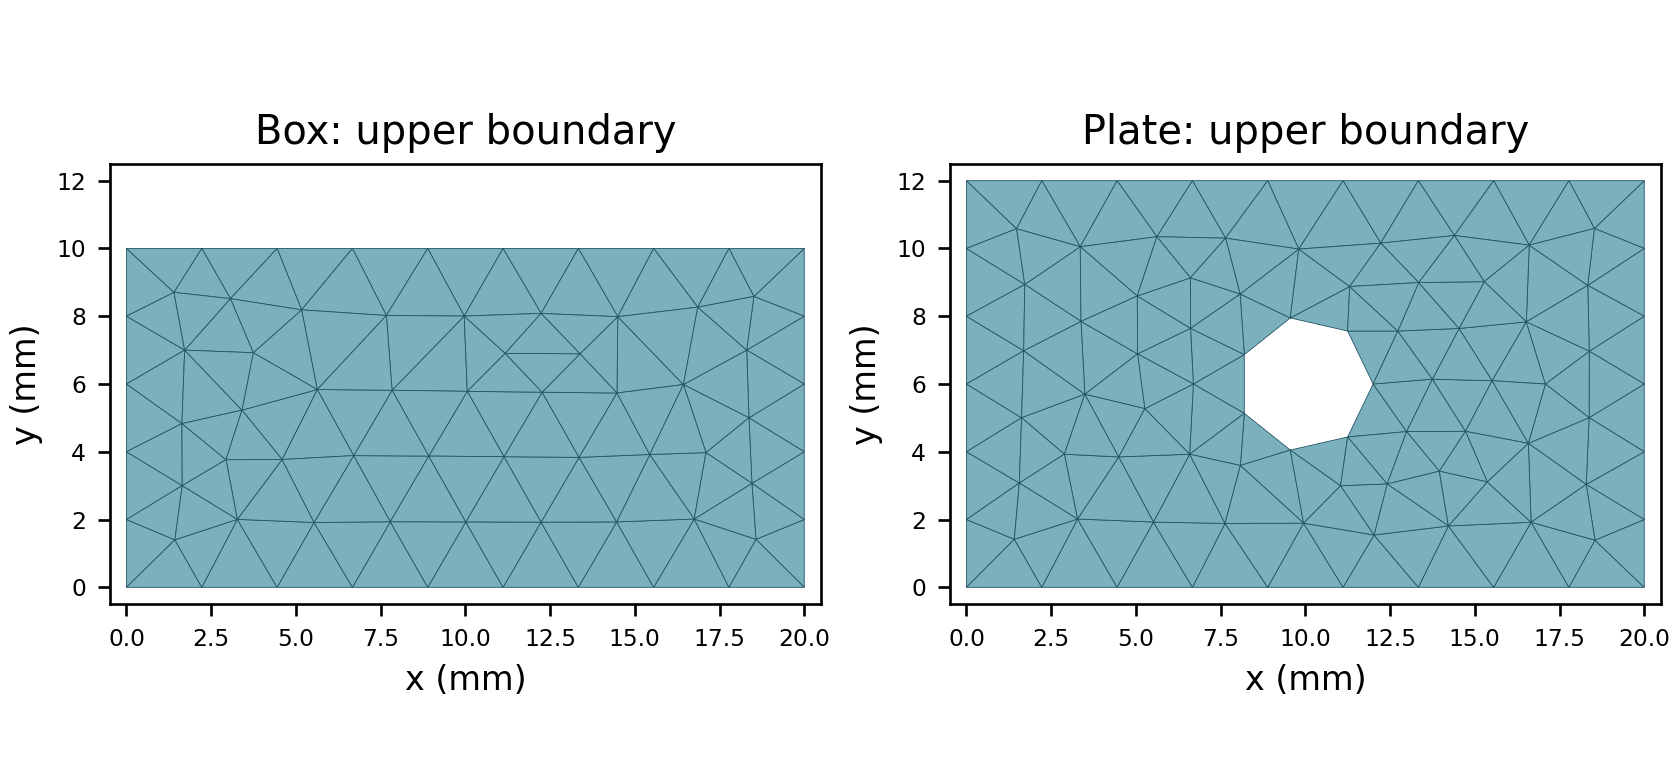
\includegraphics[width=\columnwidth]{figures/retained_boundaries.png}
\caption{Top views of the upper boundary triangles of the retained 4 mm box and plate meshes, parsed from the serialized files. All shown triangles lie at the maximum $z$ coordinate. The illustration preserves the reference extents; it is not generated geometry.}
\label{fig:reference}
\end{figure}

\section{Reproduction and Scope}
The independent analyzer uses only the Python standard library and accepts an explicit retained bundle and a new output directory. Its report binds the original summary, manifest, each mesh and its own source by SHA-256. It requires no native Gmsh installation for replay. Reproducing the original STEP-to-mesh construction is a separate command requiring the pinned native environment; byte-identical STEP headers or mesh ordering are not promised across environments.

The analyzer's nine tests exercise analytical and adversarial small complexes. They supplement the prior 195 scoped backend, serialization, CLI and reference-volume tests; those suites are different units of evidence and are not treated as 204 independent scientific replications. The protected learned-parser and VCG studies remain unchanged. No training, dataset split, new holdout or favorable parameter search occurs in this note.

Two constructed parts are appropriate for an inspectable tool example, but insufficient for a broad CAD benchmark or a regular shape-modeling journal contribution. Thin features, assemblies, mixed elements, high-order elements, alternative kernels, independent meshers, industrial inputs and solver quantities are outside this evidence. A stronger study would need a distinct question, representative permissible models and predeclared comparisons. This note provides reusable reference artifacts and a concrete failure-detection workflow on which such a study could build.

\section*{AI Assistance and Author Review}
OpenAI Codex assisted with analysis software, drafting and deterministic figures. The manuscript is prepared without author identity fields for human review. Before submission, the human authors must verify the content, finalize authorship, and approve SIAM's required responsibility statement. That approval is not asserted by this draft.

\begin{thebibliography}{9}
\bibitem{gmsh2009} C. Geuzaine and J.-F. Remacle, Gmsh: a three-dimensional finite element mesh generator with built-in pre- and post-processing facilities, \emph{International Journal for Numerical Methods in Engineering}, 79 (2009), pp. 1309--1331. \url{https://doi.org/10.1002/nme.2579}.
\bibitem{gmshmanual} C. Geuzaine and J.-F. Remacle, \emph{Gmsh Reference Manual, version 4.15.2}, 2026. Sections 6.4 and 10.1. \url{https://gmsh.info/doc/texinfo/gmsh.html}.
\end{thebibliography}
\end{document}
